%% eval.tex
%% $Id: eval.tex 61 2012-05-03 13:58:03Z bless $

\chapter{Evaluation}
\label{ch:Evaluierung}
%% ==============================
Mit verschiedenen Sweepingstrategien, Zahlentypen, Definitionsmöglichkeiten der Taylormodelle, initialer Ungenauigkeit, Genauigkeitsmodell (absolute oder relative Genauigkeit) und weiteren Einstellungsmöglichkeiten, ergibt sich ein sehr großer Suchraum zum Finden der optimalen Konfiguration für nichtlineare Taylormodelle. Allerdings ermöglichen sich dadurch sehr feingranulare Vergleiche, um herauszufinden, ob eine Implementierung nichtlinearer Taylormodelle in der Praxis schneller oder genauer als eine lineare sein kann. In diesem Kapitel werden Ergebnisse einige dieser Optionen betrachtet und versucht, die beobachteten Effekte zu erklären.

\section{Messungenauigkeiten}
\begin{align}
    x_0 &= [0 \pm 0] + [1 \pm 0] \cdot \lambda & \lambda \in [0.5 \pm \varepsilon] \label{tm1} \\ 
    x_0 &= [0.5 \pm 0] + [1 \pm 0] \cdot \lambda & \lambda \in [0 \pm \varepsilon] \label{tm2} \\
    x_0 &= [0.5 \pm 0] + [\varepsilon \pm 0] \cdot \lambda & \lambda \in [0 \pm 1] \label{tm3} \\
    x_0 &= [0 \pm 0] + [0.5 \pm \varepsilon] \cdot \lambda & \lambda \in [1 \pm 0] \label{tm4} \\
    x_0 &= [0.5 \pm 0] + [0 \pm \varepsilon] \cdot \lambda & \lambda \in [1 \pm 0] \label{tm5} \\
    x_0 &= [0.5 \pm \varepsilon] \label{tm6}
\end{align}


% 
\begin{figure}[ht]
    \centering
    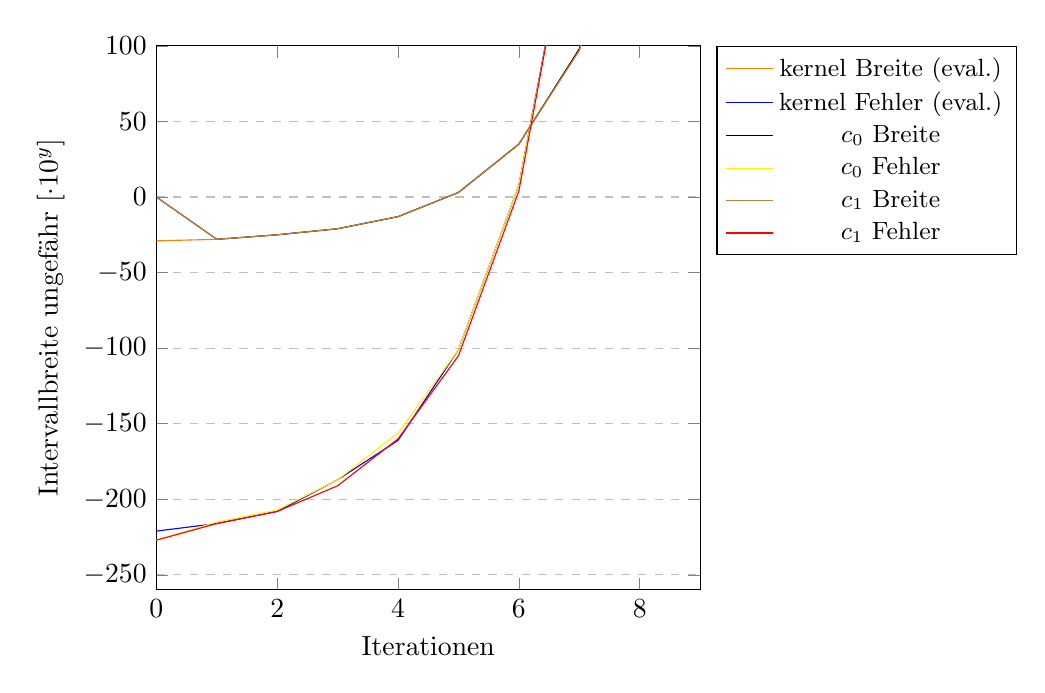
\begin{tikzpicture}
    \begin{axis}[
        width=0.7\textwidth,
        height=0.7\textwidth,
        xlabel={Iterationen},
        ylabel={Intervallbreite ungefähr $[\cdot 10^y ]$},
        legend pos=north west,
        xmin=0,xmax=9,
        ymax=100,
        ymajorgrids=true,
        grid style=dashed,
        legend pos=outer north east,
        cycle list name=color list
    ]
    
    \addplot[
        color=orange,
        ]
        coordinates {
    (0,-29)
(1,-28)
(2,-25)
(3,-21)
(4,-13)
(5,03)
(6,35)
(7,97)
(8,223)
        };
        \addlegendentry{\small{kernel Breite (eval.)}}
    
    \addplot
        coordinates {
    (0,-221)
(1,-216)
(2,-208)
(3,-187)
(4,-161)
(5,-101)
(6,8)
(7,219)
        };
        \addlegendentry{\small{kernel Fehler (eval.)}}
       
    
    \addplot
        coordinates {
    (0,0)
 (1,-28)
 (2,-25)
 (3,-21)
 (4,-13)
 (5,003)
 (6,035)
 (7,098)
 (8,223)
        };
        \addlegendentry{\small{$c_0$ Breite}}
        
    \addplot
        coordinates {
   (0,-227)
(1,-215)
(2,-207)
(3,-187)
(4,-156)
(5,-101)
(6,8)
(7,216)
(8,637)
        };
        \addlegendentry{\small{$c_0$ Fehler}}
    
        \addplot
        coordinates {
    (0,0)
 (1,-28)
 (2,-25)
 (3,-21)
 (4,-13)
 (5,+3)
 (6,+35)
 (7,+97)
 (8,+223)
        };
        \addlegendentry{\small{$c_1$ Breite}}
    
        \addplot[
        color=red,
        ]
        coordinates {
   (0,-227)
(1,-216)
(2,-208)
(3,-191)
(4,-160)
(5,-105)
(6,4)
(7,220)
        };
        \addlegendentry{\small{$c_1$ Fehler}}
    
    
    \end{axis}
    \end{tikzpicture}
    \caption{$ x_0 = [0 \pm 0] + [1 \pm 0] \cdot \lambda,\  \lambda \in [0.5 \pm \varepsilon] $}
    \label{fig:tm1}
\end{figure}
% 
\begin{figure}[ht]
    \centering
    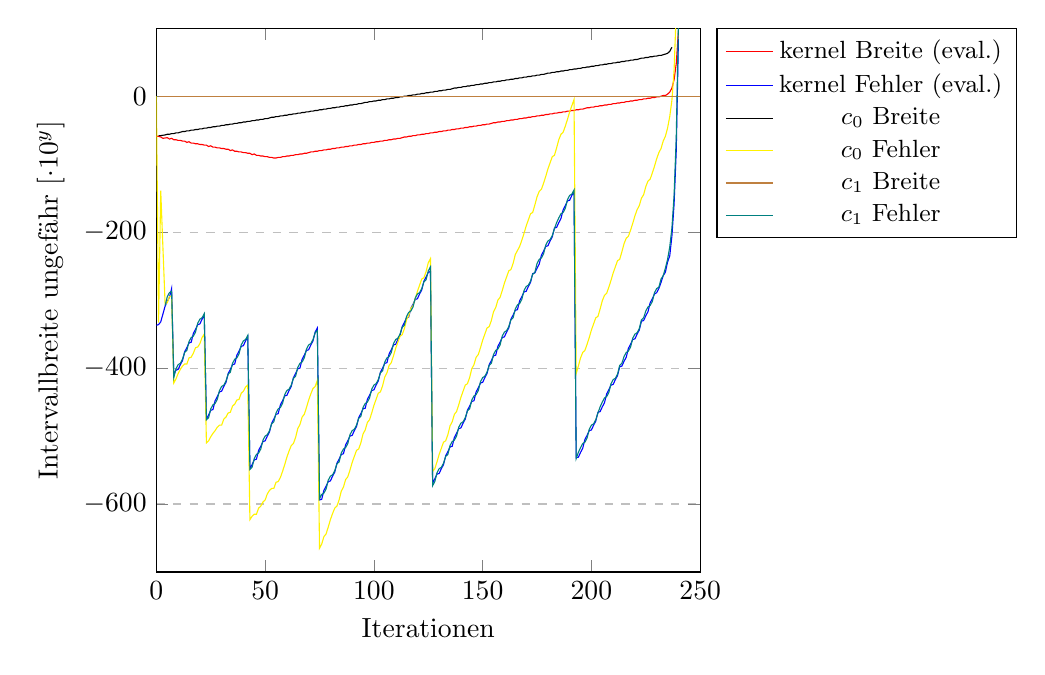
\begin{tikzpicture}
    \begin{axis}[
        width=0.7\textwidth,
        height=0.7\textwidth,
        xlabel={Iterationen},
        ylabel={Intervallbreite ungefähr $[\cdot 10^y ]$},
        legend pos=north west,
        xmin=0,xmax=250,
        ymax=100,ymin=-700,
        ymajorgrids=true,
        grid style=dashed,
        legend pos=outer north east,
        cycle list name=color list
    ]
    
    \addplot
        coordinates {
 (0,-59)
 (1,-59)
 (2,-60)
 (3,-62)
 (5,-61)
 (6,-63)
 (7,-62)
 (8,-64)
 (9,-64)
 (10,-65)
 (11,-65)
 (12,-66)
 (13,-66)
 (14,-68)
 (15,-67)
 (16,-69)
 (17,-69)
 (18,-70)
 (19,-70)
 (20,-71)
 (21,-71)
 (22,-72)
 (23,-72)
 (24,-74)
 (25,-73)
 (26,-75)
 (27,-75)
 (28,-76)
 (29,-76)
 (30,-77)
 (31,-77)
 (32,-78)
 (33,-78)
 (34,-80)
 (35,-79)
 (36,-81)
 (37,-81)
 (38,-82)
 (39,-82)
 (40,-83)
 (41,-83)
 (42,-84)
 (43,-84)
 (44,-86)
 (45,-85)
 (46,-87)
 (47,-87)
 (48,-88)
 (49,-88)
 (50,-89)
 (51,-89)
 (52,-90)
 (53,-90)
 (54,-91)
 (55,-91)
 (56,-90)
 (57,-90)
 (58,-89)
 (59,-89)
 (60,-88)
 (61,-88)
 (62,-87)
 (63,-87)
 (64,-86)
 (65,-86)
 (66,-85)
 (67,-85)
 (68,-84)
 (69,-84)
 (70,-83)
 (71,-82)
 (72,-82)
 (73,-81)
 (74,-81)
 (75,-80)
 (76,-80)
 (77,-79)
 (78,-79)
 (79,-78)
 (80,-78)
 (81,-77)
 (82,-77)
 (83,-76)
 (84,-76)
 (85,-75)
 (86,-75)
 (87,-74)
 (88,-74)
 (89,-73)
 (90,-73)
 (91,-72)
 (92,-72)
 (93,-71)
 (94,-71)
 (95,-70)
 (96,-70)
 (97,-69)
 (98,-69)
 (99,-68)
 (100,-68)
 (101,-67)
 (102,-67)
 (103,-66)
 (104,-66)
 (105,-65)
 (106,-65)
 (107,-64)
 (108,-64)
 (109,-63)
 (110,-63)
 (111,-62)
 (112,-62)
 (113,-61)
 (114,-60)
 (115,-60)
 (116,-59)
 (117,-59)
 (118,-58)
 (119,-58)
 (120,-57)
 (121,-57)
 (122,-56)
 (123,-56)
 (124,-55)
 (125,-55)
 (126,-54)
 (127,-54)
 (128,-53)
 (129,-53)
 (130,-52)
 (131,-52)
 (132,-51)
 (133,-51)
 (134,-50)
 (135,-50)
 (136,-49)
 (137,-49)
 (138,-48)
 (139,-48)
 (140,-47)
 (141,-47)
 (142,-46)
 (143,-46)
 (144,-45)
 (145,-45)
 (146,-44)
 (147,-44)
 (148,-43)
 (149,-43)
 (150,-42)
 (151,-42)
 (152,-41)
 (153,-41)
 (154,-40)
 (155,-39)
 (156,-39)
 (157,-38)
 (158,-38)
 (159,-37)
 (160,-37)
 (161,-36)
 (162,-36)
 (163,-35)
 (164,-35)
 (165,-34)
 (166,-34)
 (167,-33)
 (168,-33)
 (169,-32)
 (170,-32)
 (171,-31)
 (172,-31)
 (173,-30)
 (174,-30)
 (175,-29)
 (176,-29)
 (177,-28)
 (178,-28)
 (179,-27)
 (180,-27)
 (181,-26)
 (182,-26)
 (183,-25)
 (184,-25)
 (185,-24)
 (186,-24)
 (187,-23)
 (188,-23)
 (189,-22)
 (190,-22)
 (191,-21)
 (192,-21)
 (193,-20)
 (194,-20)
 (195,-19)
 (196,-19)
 (197,-18)
 (198,-17)
 (199,-17)
 (200,-16)
 (201,-16)
 (202,-15)
 (203,-15)
 (204,-14)
 (205,-14)
 (206,-13)
 (207,-13)
 (208,-12)
 (209,-12)
 (210,-11)
 (211,-11)
 (212,-10)
 (213,-10)
 (214,-9)
 (215,-9)
 (216,-8)
 (217,-8)
 (218,-7)
 (219,-7)
 (220,-6)
 (221,-6)
 (222,-5)
 (223,-5)
 (224,-4)
 (225,-4)
 (226,-3)
 (227,-3)
 (228,-2)
 (229,-2)
 (230,-1)
 (231,-1)
 (232,0)
 (233,1)
 (234,1)
 (235,3)
 (236,6)
 (237,12)
 (238,24)
 (239,48)
 (240,96)
        };
        \addlegendentry{\small{kernel Breite (eval.)}}
    
    \addplot
        coordinates {
(0,-337)
(1,-336)
(2,-332)
(4,-309)
(5,-302)
(6,-296)
(7,-283)
(8,-410)
(9,-403)
(10,-402)
(11,-395)
(12,-389)
(13,-376)
(14,-370)
(15,-363)
(16,-362)
(17,-349)
(18,-343)
(19,-336)
(20,-335)
(21,-328)
(22,-322)
(23,-475)
(24,-469)
(25,-462)
(26,-461)
(27,-448)
(28,-442)
(29,-435)
(30,-434)
(31,-427)
(32,-421)
(33,-408)
(34,-402)
(35,-395)
(36,-394)
(37,-381)
(38,-375)
(39,-368)
(40,-367)
(41,-360)
(42,-354)
(43,-548)
(44,-542)
(45,-535)
(46,-534)
(47,-521)
(48,-515)
(49,-508)
(50,-507)
(51,-500)
(52,-494)
(53,-481)
(54,-475)
(55,-468)
(56,-467)
(57,-454)
(58,-448)
(59,-441)
(60,-440)
(61,-433)
(62,-427)
(63,-414)
(64,-408)
(65,-401)
(66,-400)
(67,-387)
(68,-381)
(69,-374)
(70,-373)
(71,-366)
(72,-360)
(73,-347)
(74,-341)
(75,-594)
(76,-593)
(77,-580)
(78,-574)
(79,-567)
(80,-566)
(81,-559)
(82,-553)
(83,-540)
(84,-534)
(85,-527)
(86,-526)
(87,-513)
(88,-507)
(89,-500)
(90,-499)
(91,-492)
(92,-486)
(93,-473)
(94,-467)
(95,-460)
(96,-459)
(97,-446)
(98,-440)
(99,-433)
(100,-432)
(101,-425)
(102,-419)
(103,-406)
(104,-400)
(105,-393)
(106,-392)
(107,-379)
(108,-373)
(109,-366)
(110,-365)
(111,-358)
(112,-352)
(113,-339)
(114,-333)
(115,-326)
(116,-325)
(117,-312)
(118,-306)
(119,-299)
(120,-298)
(121,-291)
(122,-285)
(123,-272)
(124,-266)
(125,-259)
(126,-258)
(127,-569)
(128,-563)
(129,-556)
(130,-555)
(131,-548)
(132,-542)
(133,-529)
(134,-523)
(135,-516)
(136,-515)
(137,-502)
(138,-496)
(139,-489)
(140,-488)
(141,-481)
(142,-475)
(143,-462)
(144,-456)
(145,-449)
(146,-448)
(147,-435)
(148,-429)
(149,-422)
(150,-421)
(151,-414)
(152,-408)
(153,-395)
(154,-389)
(155,-382)
(156,-381)
(157,-368)
(158,-362)
(159,-355)
(160,-354)
(161,-347)
(162,-341)
(163,-328)
(164,-322)
(165,-315)
(166,-314)
(167,-301)
(168,-295)
(169,-288)
(170,-287)
(171,-280)
(172,-274)
(173,-261)
(174,-260)
(175,-253)
(176,-247)
(177,-234)
(178,-228)
(179,-221)
(180,-220)
(181,-213)
(182,-207)
(183,-194)
(184,-193)
(185,-186)
(186,-180)
(187,-167)
(188,-161)
(189,-154)
(190,-153)
(191,-146)
(192,-140)
(193,-532)
(194,-531)
(195,-524)
(196,-518)
(197,-505)
(198,-499)
(199,-492)
(200,-491)
(201,-484)
(202,-478)
(203,-465)
(204,-464)
(205,-457)
(206,-451)
(207,-438)
(208,-432)
(209,-425)
(210,-424)
(211,-417)
(212,-411)
(213,-398)
(214,-397)
(215,-390)
(216,-384)
(217,-371)
(218,-365)
(219,-358)
(220,-357)
(221,-350)
(222,-344)
(223,-331)
(224,-330)
(225,-323)
(226,-317)
(227,-304)
(228,-298)
(229,-291)
(230,-289)
(231,-283)
(232,-274)
(233,-264)
(234,-259)
(235,-244)
(236,-235)
(237,-206)
(238,-159)
(239,-80)
(240,84)
        };
        \addlegendentry{\small{kernel Fehler (eval.)}}
       
    
    \addplot
        coordinates {
(1,-58)
(2,-58)
(4,-57)
(5,-56)
(6,-56)
(7,-55)
(8,-55)
(9,-54)
(10,-54)
(11,-53)
(12,-52)
(13,-52)
(14,-51)
(15,-51)
(16,-50)
(17,-50)
(18,-49)
(19,-49)
(20,-48)
(21,-48)
(22,-47)
(23,-47)
(24,-46)
(25,-46)
(26,-45)
(27,-45)
(28,-44)
(29,-44)
(30,-43)
(31,-43)
(32,-42)
(33,-42)
(34,-41)
(35,-41)
(36,-40)
(37,-40)
(38,-39)
(39,-39)
(40,-38)
(41,-38)
(42,-37)
(43,-37)
(44,-36)
(45,-36)
(46,-35)
(47,-35)
(48,-34)
(49,-34)
(50,-33)
(51,-33)
(52,-32)
(53,-31)
(54,-31)
(55,-30)
(56,-30)
(57,-29)
(58,-29)
(59,-28)
(60,-28)
(61,-27)
(62,-27)
(63,-26)
(64,-26)
(65,-25)
(66,-25)
(67,-24)
(68,-24)
(69,-23)
(70,-23)
(71,-22)
(72,-22)
(73,-21)
(74,-21)
(75,-20)
(76,-20)
(77,-19)
(78,-19)
(79,-18)
(80,-18)
(81,-17)
(82,-17)
(83,-16)
(84,-16)
(85,-15)
(86,-15)
(87,-14)
(88,-14)
(89,-13)
(90,-13)
(91,-12)
(92,-12)
(93,-11)
(94,-11)
(95,-10)
(96,-9)
(97,-9)
(98,-8)
(99,-8)
(100,-7)
(101,-7)
(102,-6)
(103,-6)
(104,-5)
(105,-5)
(106,-4)
(107,-4)
(108,-3)
(109,-3)
(110,-2)
(111,-2)
(112,-1)
(113,-1)
(114,0)
(115,0)
(116,1)
(117,1)
(118,2)
(119,2)
(120,3)
(121,3)
(122,4)
(123,4)
(124,5)
(125,5)
(126,6)
(127,6)
(128,7)
(129,7)
(130,8)
(131,8)
(132,9)
(133,9)
(134,10)
(135,10)
(136,11)
(137,12)
(138,12)
(139,13)
(140,13)
(141,14)
(142,14)
(143,15)
(144,15)
(145,16)
(146,16)
(147,17)
(148,17)
(149,18)
(150,18)
(151,19)
(152,19)
(153,20)
(154,20)
(155,21)
(156,21)
(157,22)
(158,22)
(159,23)
(160,23)
(161,24)
(162,24)
(163,25)
(164,25)
(165,26)
(166,26)
(167,27)
(168,27)
(169,28)
(170,28)
(171,29)
(172,29)
(173,30)
(174,30)
(175,31)
(176,31)
(177,32)
(178,32)
(179,33)
(180,34)
(181,34)
(182,35)
(183,35)
(184,36)
(185,36)
(186,37)
(187,37)
(188,38)
(189,38)
(190,39)
(191,39)
(192,40)
(193,40)
(194,41)
(195,41)
(196,42)
(197,42)
(198,43)
(199,43)
(200,44)
(201,44)
(202,45)
(203,45)
(204,46)
(205,46)
(206,47)
(207,47)
(208,48)
(209,48)
(210,49)
(211,49)
(212,50)
(213,50)
(214,51)
(215,51)
(216,52)
(217,52)
(218,53)
(219,53)
(220,54)
(221,54)
(222,55)
(223,56)
(224,56)
(225,57)
(226,57)
(227,58)
(228,58)
(229,59)
(230,59)
(231,60)
(232,60)
(233,61)
(234,62)
(235,63)
(236,66)
(237,72)
        };
        \addlegendentry{\small{$c_0$ Breite}}
        
    \addplot
        coordinates {
 (0,0)
 (1,-333)
 (2,-139)
 (4,-305)
 (5,-304)
 (6,-295)
 (7,-294)
 (8,-422)
 (9,-416)
 (10,-408)
 (11,-402)
 (12,-397)
 (13,-394)
 (14,-394)
 (15,-385)
 (16,-384)
 (17,-378)
 (18,-370)
 (19,-369)
 (20,-364)
 (21,-355)
 (22,-350)
 (23,-510)
 (24,-507)
 (25,-501)
 (26,-496)
 (27,-492)
 (28,-487)
 (29,-484)
 (30,-484)
 (31,-475)
 (32,-472)
 (33,-466)
 (34,-465)
 (35,-456)
 (36,-453)
 (37,-447)
 (38,-446)
 (39,-437)
 (40,-434)
 (41,-428)
 (42,-425)
 (43,-623)
 (44,-618)
 (45,-615)
 (46,-615)
 (47,-606)
 (48,-603)
 (49,-597)
 (50,-594)
 (51,-585)
 (52,-580)
 (53,-577)
 (54,-577)
 (55,-568)
 (56,-567)
 (57,-561)
 (58,-552)
 (59,-542)
 (60,-531)
 (61,-522)
 (62,-514)
 (63,-511)
 (64,-502)
 (65,-489)
 (66,-483)
 (67,-472)
 (68,-468)
 (69,-458)
 (70,-447)
 (71,-438)
 (72,-430)
 (73,-427)
 (74,-418)
 (75,-665)
 (76,-659)
 (77,-648)
 (78,-644)
 (79,-634)
 (80,-623)
 (81,-614)
 (82,-606)
 (83,-603)
 (84,-594)
 (85,-581)
 (86,-575)
 (87,-564)
 (88,-560)
 (89,-550)
 (90,-539)
 (91,-530)
 (92,-521)
 (93,-519)
 (94,-510)
 (95,-497)
 (96,-491)
 (97,-480)
 (98,-476)
 (99,-466)
 (100,-455)
 (101,-446)
 (102,-437)
 (103,-435)
 (104,-426)
 (105,-413)
 (106,-407)
 (107,-396)
 (108,-392)
 (109,-382)
 (110,-371)
 (111,-362)
 (112,-353)
 (113,-351)
 (114,-342)
 (115,-329)
 (116,-323)
 (117,-312)
 (118,-308)
 (119,-298)
 (120,-287)
 (121,-278)
 (122,-269)
 (123,-267)
 (124,-258)
 (125,-245)
 (126,-239)
 (127,-552)
 (128,-548)
 (129,-538)
 (130,-527)
 (131,-518)
 (132,-509)
 (133,-507)
 (134,-498)
 (135,-485)
 (136,-479)
 (137,-468)
 (138,-464)
 (139,-454)
 (140,-443)
 (141,-434)
 (142,-425)
 (143,-423)
 (144,-414)
 (145,-401)
 (146,-395)
 (147,-384)
 (148,-380)
 (149,-370)
 (150,-359)
 (151,-350)
 (152,-341)
 (153,-339)
 (154,-330)
 (155,-317)
 (156,-311)
 (157,-300)
 (158,-296)
 (159,-286)
 (160,-275)
 (161,-266)
 (162,-257)
 (163,-255)
 (164,-246)
 (165,-233)
 (166,-227)
 (167,-221)
 (168,-212)
 (169,-202)
 (170,-191)
 (171,-182)
 (172,-173)
 (173,-171)
 (174,-160)
 (175,-148)
 (176,-140)
 (177,-137)
 (178,-128)
 (179,-118)
 (180,-107)
 (181,-98)
 (182,-89)
 (183,-87)
 (184,-76)
 (185,-64)
 (186,-56)
 (187,-53)
 (188,-44)
 (189,-34)
 (190,-23)
 (191,-14)
 (192,-5)
 (193,-408)
 (194,-397)
 (195,-385)
 (196,-377)
 (197,-374)
 (198,-365)
 (199,-355)
 (200,-344)
 (201,-335)
 (202,-326)
 (203,-324)
 (204,-313)
 (205,-301)
 (206,-293)
 (207,-290)
 (208,-281)
 (209,-271)
 (210,-260)
 (211,-251)
 (212,-242)
 (213,-240)
 (214,-229)
 (215,-217)
 (216,-209)
 (217,-206)
 (218,-197)
 (219,-187)
 (220,-176)
 (221,-167)
 (222,-161)
 (223,-150)
 (224,-145)
 (225,-133)
 (226,-125)
 (227,-122)
 (228,-113)
 (229,-103)
 (230,-92)
 (231,-83)
 (232,-77)
 (233,-66)
 (234,-59)
 (235,-47)
 (236,-30)
 (237,-6)
 (238,38)
 (239,125)
        };
        \addlegendentry{\small{$c_0$ Fehler}}
    
        \addplot
        coordinates {
 (1,0)
 (2,0)
 (4,0)
 (5,0)
 (6,0)
 (7,0)
 (8,0)
 (9,0)
 (10,0)
 (11,0)
 (12,0)
 (13,0)
 (14,0)
 (15,0)
 (16,0)
 (17,0)
 (18,0)
 (19,0)
 (20,0)
 (21,0)
 (22,0)
 (23,0)
 (24,0)
 (25,0)
 (26,0)
 (27,0)
 (28,0)
 (29,0)
 (30,0)
 (31,0)
 (32,0)
 (33,0)
 (34,0)
 (35,0)
 (36,0)
 (37,0)
 (38,0)
 (39,0)
 (40,0)
 (41,0)
 (42,0)
 (43,0)
 (44,0)
 (45,0)
 (46,0)
 (47,0)
 (48,0)
 (49,0)
 (50,0)
 (51,0)
 (52,0)
 (53,0)
 (54,0)
 (55,0)
 (56,0)
 (57,0)
 (58,0)
 (59,0)
 (60,0)
 (61,0)
 (62,0)
 (63,0)
 (64,0)
 (65,0)
 (66,0)
 (67,0)
 (68,0)
 (69,0)
 (70,0)
 (71,0)
 (72,0)
 (73,0)
 (74,0)
 (75,0)
 (76,0)
 (77,0)
 (78,0)
 (79,0)
 (80,0)
 (81,0)
 (82,0)
 (83,0)
 (84,0)
 (85,0)
 (86,0)
 (87,0)
 (88,0)
 (89,0)
 (90,0)
 (91,0)
 (92,0)
 (93,0)
 (94,0)
 (95,0)
 (96,0)
 (97,0)
 (98,0)
 (99,0)
 (100,0)
 (101,0)
 (102,0)
 (103,0)
 (104,0)
 (105,0)
 (106,0)
 (107,0)
 (108,0)
 (109,0)
 (110,0)
 (111,0)
 (112,0)
 (113,0)
 (114,0)
 (115,0)
 (116,0)
 (117,0)
 (118,0)
 (119,0)
 (120,0)
 (121,0)
 (122,0)
 (123,0)
 (124,0)
 (125,0)
 (126,0)
 (127,0)
 (128,0)
 (129,0)
 (130,0)
 (131,0)
 (132,0)
 (133,0)
 (134,0)
 (135,0)
 (136,0)
 (137,0)
 (138,0)
 (139,0)
 (140,0)
 (141,0)
 (142,0)
 (143,0)
 (144,0)
 (145,0)
 (146,0)
 (147,0)
 (148,0)
 (149,0)
 (150,0)
 (151,0)
 (152,0)
 (153,0)
 (154,0)
 (155,0)
 (156,0)
 (157,0)
 (158,0)
 (159,0)
 (160,0)
 (161,0)
 (162,0)
 (163,0)
 (164,0)
 (165,0)
 (166,0)
 (167,0)
 (168,0)
 (169,0)
 (170,0)
 (171,0)
 (172,0)
 (173,0)
 (174,0)
 (175,0)
 (176,0)
 (177,0)
 (178,0)
 (179,0)
 (180,0)
 (181,0)
 (182,0)
 (183,0)
 (184,0)
 (185,0)
 (186,0)
 (187,0)
 (188,0)
 (189,0)
 (190,0)
 (191,0)
 (192,0)
 (193,0)
 (194,0)
 (195,0)
 (196,0)
 (197,0)
 (198,0)
 (199,0)
 (200,0)
 (201,0)
 (202,0)
 (203,0)
 (204,0)
 (205,0)
 (206,0)
 (207,0)
 (208,0)
 (209,0)
 (210,0)
 (211,0)
 (212,0)
 (213,0)
 (214,0)
 (215,0)
 (216,0)
 (217,0)
 (218,0)
 (219,0)
 (220,0)
 (221,0)
 (222,0)
 (223,0)
 (224,0)
 (225,0)
 (226,0)
 (227,0)
 (228,0)
 (229,0)
 (230,0)
 (231,0)
 (232,0)
 (233,0)
 (234,0)
 (235,0)
 (236,0)
 (237,0)
 (238,0)
 (239,0)
 (240,0)
 (241,0)
 (242,0)
 (243,0)
 (244,0)
 (245,0)
 (246,0)
 (247,0)
 (248,0)
 (249,0)
 (250,0)
        };
        \addlegendentry{\small{$c_1$ Breite}}
    
        \addplot
        coordinates {
 (4,-308)
 (5,-295)
 (6,-289)
 (7,-287)
 (8,-414)
 (9,-401)
 (10,-395)
 (11,-393)
 (12,-387)
 (13,-377)
 (14,-374)
 (15,-361)
 (16,-355)
 (17,-353)
 (18,-347)
 (19,-334)
 (20,-328)
 (21,-326)
 (22,-320)
 (23,-476)
 (24,-473)
 (25,-460)
 (26,-454)
 (27,-452)
 (28,-446)
 (29,-433)
 (30,-427)
 (31,-425)
 (32,-419)
 (33,-409)
 (34,-406)
 (35,-393)
 (36,-387)
 (37,-385)
 (38,-379)
 (39,-366)
 (40,-360)
 (41,-358)
 (42,-352)
 (43,-549)
 (44,-546)
 (45,-533)
 (46,-527)
 (47,-525)
 (48,-519)
 (49,-506)
 (50,-500)
 (51,-498)
 (52,-492)
 (53,-482)
 (54,-479)
 (55,-466)
 (56,-460)
 (57,-458)
 (58,-452)
 (59,-439)
 (60,-433)
 (61,-431)
 (62,-425)
 (63,-415)
 (64,-412)
 (65,-399)
 (66,-393)
 (67,-391)
 (68,-385)
 (69,-372)
 (70,-366)
 (71,-364)
 (72,-358)
 (73,-348)
 (74,-345)
 (75,-592)
 (76,-586)
 (77,-584)
 (78,-578)
 (79,-565)
 (80,-559)
 (81,-557)
 (82,-551)
 (83,-541)
 (84,-538)
 (85,-525)
 (86,-519)
 (87,-517)
 (88,-511)
 (89,-498)
 (90,-492)
 (91,-490)
 (92,-484)
 (93,-474)
 (94,-471)
 (95,-458)
 (96,-452)
 (97,-450)
 (98,-444)
 (99,-431)
 (100,-425)
 (101,-423)
 (102,-417)
 (103,-407)
 (104,-404)
 (105,-391)
 (106,-385)
 (107,-383)
 (108,-377)
 (109,-364)
 (110,-358)
 (111,-356)
 (112,-350)
 (113,-340)
 (114,-337)
 (115,-324)
 (116,-318)
 (117,-316)
 (118,-310)
 (119,-297)
 (120,-291)
 (121,-289)
 (122,-283)
 (123,-273)
 (124,-270)
 (125,-257)
 (126,-251)
 (127,-573)
 (128,-567)
 (129,-554)
 (130,-548)
 (131,-546)
 (132,-540)
 (133,-530)
 (134,-527)
 (135,-514)
 (136,-508)
 (137,-506)
 (138,-500)
 (139,-487)
 (140,-481)
 (141,-479)
 (142,-473)
 (143,-463)
 (144,-460)
 (145,-447)
 (146,-441)
 (147,-439)
 (148,-433)
 (149,-420)
 (150,-414)
 (151,-412)
 (152,-406)
 (153,-396)
 (154,-393)
 (155,-380)
 (156,-374)
 (157,-372)
 (158,-366)
 (159,-353)
 (160,-347)
 (161,-345)
 (162,-339)
 (163,-329)
 (164,-326)
 (165,-313)
 (166,-307)
 (167,-305)
 (168,-299)
 (169,-286)
 (170,-280)
 (171,-278)
 (172,-272)
 (173,-262)
 (174,-259)
 (175,-246)
 (176,-240)
 (177,-238)
 (178,-232)
 (179,-219)
 (180,-213)
 (181,-211)
 (182,-205)
 (183,-195)
 (184,-186)
 (185,-179)
 (186,-173)
 (187,-171)
 (188,-165)
 (189,-152)
 (190,-146)
 (191,-144)
 (192,-138)
 (193,-533)
 (194,-524)
 (195,-517)
 (196,-511)
 (197,-509)
 (198,-503)
 (199,-490)
 (200,-484)
 (201,-482)
 (202,-476)
 (203,-466)
 (204,-457)
 (205,-450)
 (206,-444)
 (207,-442)
 (208,-436)
 (209,-423)
 (210,-417)
 (211,-415)
 (212,-409)
 (213,-396)
 (214,-393)
 (215,-383)
 (216,-377)
 (217,-375)
 (218,-369)
 (219,-356)
 (220,-350)
 (221,-348)
 (222,-342)
 (223,-329)
 (224,-326)
 (225,-316)
 (226,-310)
 (227,-308)
 (228,-302)
 (229,-289)
 (230,-283)
 (231,-281)
 (232,-269)
 (233,-264)
 (234,-253)
 (235,-240)
 (236,-222)
 (237,-194)
 (238,-146)
 (239,-60)
 (240,108)
 (241,436)
        };
        \addlegendentry{\small{$c_1$ Fehler}}
    
    
    \end{axis}
    \end{tikzpicture}
    \caption{$x_0 = [0.5 \pm 0] + [1 \pm 0] \cdot \lambda,\  \lambda \in [0 \pm \varepsilon]$}
    \label{fig:tm2}
\end{figure}
% 
\begin{figure}[ht]
    \centering
    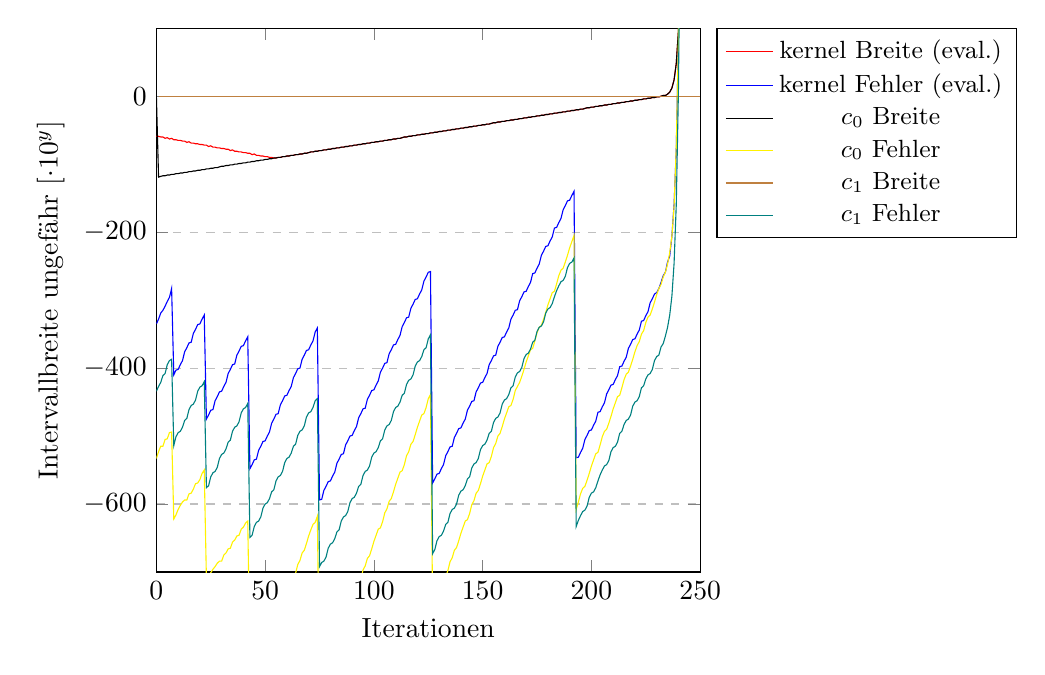
\begin{tikzpicture}
    \begin{axis}[
        width=0.7\textwidth,
        height=0.7\textwidth,
        xlabel={Iterationen},
        ylabel={Intervallbreite ungefähr $[\cdot 10^y ]$},
        legend pos=north west,
        xmin=0,xmax=250,
        ymax=100,ymin=-700,
        ymajorgrids=true,
        grid style=dashed,
        legend pos=outer north east,
        cycle list name=color list
    ]
    
    \addplot
        coordinates {
  (0,-59)
 (1,-59)
 (2,-60)
 (3,-60)
 (4,-62)
 (5,-61)
 (6,-63)
 (7,-62)
 (8,-64)
 (9,-64)
 (10,-65)
 (11,-65)
 (12,-66)
 (13,-66)
 (14,-68)
 (15,-67)
 (16,-69)
 (17,-69)
 (18,-70)
 (19,-70)
 (20,-71)
 (21,-71)
 (22,-72)
 (23,-72)
 (24,-74)
 (25,-73)
 (26,-75)
 (27,-75)
 (28,-76)
 (29,-76)
 (30,-77)
 (31,-77)
 (32,-78)
 (33,-78)
 (34,-80)
 (35,-79)
 (36,-81)
 (37,-81)
 (38,-82)
 (39,-82)
 (40,-83)
 (41,-83)
 (42,-84)
 (43,-84)
 (44,-86)
 (45,-85)
 (46,-87)
 (47,-87)
 (48,-88)
 (49,-88)
 (50,-89)
 (51,-89)
 (52,-90)
 (53,-90)
 (54,-91)
 (55,-91)
 (56,-90)
 (57,-90)
 (58,-89)
 (59,-89)
 (60,-88)
 (61,-88)
 (62,-87)
 (63,-87)
 (64,-86)
 (65,-86)
 (66,-85)
 (67,-85)
 (68,-84)
 (69,-84)
 (70,-83)
 (71,-82)
 (72,-82)
 (73,-81)
 (74,-81)
 (75,-80)
 (76,-80)
 (77,-79)
 (78,-79)
 (79,-78)
 (80,-78)
 (81,-77)
 (82,-77)
 (83,-76)
 (84,-76)
 (85,-75)
 (86,-75)
 (87,-74)
 (88,-74)
 (89,-73)
 (90,-73)
 (91,-72)
 (92,-72)
 (93,-71)
 (94,-71)
 (95,-70)
 (96,-70)
 (97,-69)
 (98,-69)
 (99,-68)
 (100,-68)
 (101,-67)
 (102,-67)
 (103,-66)
 (104,-66)
 (105,-65)
 (106,-65)
 (107,-64)
 (108,-64)
 (109,-63)
 (110,-63)
 (111,-62)
 (112,-62)
 (113,-61)
 (114,-60)
 (115,-60)
 (116,-59)
 (117,-59)
 (118,-58)
 (119,-58)
 (120,-57)
 (121,-57)
 (122,-56)
 (123,-56)
 (124,-55)
 (125,-55)
 (126,-54)
 (127,-54)
 (128,-53)
 (129,-53)
 (130,-52)
 (131,-52)
 (132,-51)
 (133,-51)
 (134,-50)
 (135,-50)
 (136,-49)
 (137,-49)
 (138,-48)
 (139,-48)
 (140,-47)
 (141,-47)
 (142,-46)
 (143,-46)
 (144,-45)
 (145,-45)
 (146,-44)
 (147,-44)
 (148,-43)
 (149,-43)
 (150,-42)
 (151,-42)
 (152,-41)
 (153,-41)
 (154,-40)
 (155,-39)
 (156,-39)
 (157,-38)
 (158,-38)
 (159,-37)
 (160,-37)
 (161,-36)
 (162,-36)
 (163,-35)
 (164,-35)
 (165,-34)
 (166,-34)
 (167,-33)
 (168,-33)
 (169,-32)
 (170,-32)
 (171,-31)
 (172,-31)
 (173,-30)
 (174,-30)
 (175,-29)
 (176,-29)
 (177,-28)
 (178,-28)
 (179,-27)
 (180,-27)
 (181,-26)
 (182,-26)
 (183,-25)
 (184,-25)
 (185,-24)
 (186,-24)
 (187,-23)
 (188,-23)
 (189,-22)
 (190,-22)
 (191,-21)
 (192,-21)
 (193,-20)
 (194,-20)
 (195,-19)
 (196,-19)
 (197,-18)
 (198,-17)
 (199,-17)
 (200,-16)
 (201,-16)
 (202,-15)
 (203,-15)
 (204,-14)
 (205,-14)
 (206,-13)
 (207,-13)
 (208,-12)
 (209,-12)
 (210,-11)
 (211,-11)
 (212,-10)
 (213,-10)
 (214,-9)
 (215,-9)
 (216,-8)
 (217,-8)
 (218,-7)
 (219,-7)
 (220,-6)
 (221,-6)
 (222,-5)
 (223,-5)
 (224,-4)
 (225,-4)
 (226,-3)
 (227,-3)
 (228,-2)
 (229,-2)
 (230,-1)
 (231,-1)
 (232,0)
 (233,01)
 (234,01)
 (235,03)
 (236,06)
 (237,012)
 (238,024)
 (239,048)
 (240,096)
 (241,0192)
        };
        \addlegendentry{\small{kernel Breite (eval.)}}
    
    \addplot
        coordinates {
 (0,-335)
 (1,-328)
 (2,-319)
 (3,-315)
 (4,-309)
 (5,-302)
 (6,-296)
 (7,-283)
 (8,-410)
 (9,-403)
 (10,-402)
 (11,-395)
 (12,-389)
 (13,-376)
 (14,-370)
 (15,-363)
 (16,-362)
 (17,-349)
 (18,-343)
 (19,-336)
 (20,-335)
 (21,-328)
 (22,-322)
 (23,-475)
 (24,-469)
 (25,-462)
 (26,-461)
 (27,-448)
 (28,-442)
 (29,-435)
 (30,-434)
 (31,-427)
 (32,-421)
 (33,-408)
 (34,-402)
 (35,-395)
 (36,-394)
 (37,-381)
 (38,-375)
 (39,-368)
 (40,-367)
 (41,-360)
 (42,-354)
 (43,-548)
 (44,-542)
 (45,-535)
 (46,-534)
 (47,-521)
 (48,-515)
 (49,-508)
 (50,-507)
 (51,-500)
 (52,-494)
 (53,-481)
 (54,-475)
 (55,-468)
 (56,-467)
 (57,-454)
 (58,-448)
 (59,-441)
 (60,-440)
 (61,-433)
 (62,-427)
 (63,-414)
 (64,-408)
 (65,-401)
 (66,-400)
 (67,-387)
 (68,-381)
 (69,-374)
 (70,-373)
 (71,-366)
 (72,-360)
 (73,-347)
 (74,-341)
 (75,-594)
 (76,-593)
 (77,-580)
 (78,-574)
 (79,-567)
 (80,-566)
 (81,-559)
 (82,-553)
 (83,-540)
 (84,-534)
 (85,-527)
 (86,-526)
 (87,-513)
 (88,-507)
 (89,-500)
 (90,-499)
 (91,-492)
 (92,-486)
 (93,-473)
 (94,-467)
 (95,-460)
 (96,-459)
 (97,-446)
 (98,-440)
 (99,-433)
 (100,-432)
 (101,-425)
 (102,-419)
 (103,-406)
 (104,-400)
 (105,-393)
 (106,-392)
 (107,-379)
 (108,-373)
 (109,-366)
 (110,-365)
 (111,-358)
 (112,-352)
 (113,-339)
 (114,-333)
 (115,-326)
 (116,-325)
 (117,-312)
 (118,-306)
 (119,-299)
 (120,-298)
 (121,-291)
 (122,-285)
 (123,-272)
 (124,-266)
 (125,-259)
 (126,-258)
 (127,-569)
 (128,-563)
 (129,-556)
 (130,-555)
 (131,-548)
 (132,-542)
 (133,-529)
 (134,-523)
 (135,-516)
 (136,-515)
 (137,-502)
 (138,-496)
 (139,-489)
 (140,-488)
 (141,-481)
 (142,-475)
 (143,-462)
 (144,-456)
 (145,-449)
 (146,-448)
 (147,-435)
 (148,-429)
 (149,-422)
 (150,-421)
 (151,-414)
 (152,-408)
 (153,-395)
 (154,-389)
 (155,-382)
 (156,-381)
 (157,-368)
 (158,-362)
 (159,-355)
 (160,-354)
 (161,-347)
 (162,-341)
 (163,-328)
 (164,-322)
 (165,-315)
 (166,-314)
 (167,-301)
 (168,-295)
 (169,-288)
 (170,-287)
 (171,-280)
 (172,-274)
 (173,-261)
 (174,-260)
 (175,-253)
 (176,-247)
 (177,-234)
 (178,-228)
 (179,-221)
 (180,-220)
 (181,-213)
 (182,-207)
 (183,-194)
 (184,-193)
 (185,-186)
 (186,-180)
 (187,-167)
 (188,-161)
 (189,-154)
 (190,-153)
 (191,-146)
 (192,-140)
 (193,-532)
 (194,-531)
 (195,-524)
 (196,-518)
 (197,-505)
 (198,-499)
 (199,-492)
 (200,-491)
 (201,-484)
 (202,-478)
 (203,-465)
 (204,-464)
 (205,-457)
 (206,-451)
 (207,-438)
 (208,-432)
 (209,-425)
 (210,-424)
 (211,-417)
 (212,-411)
 (213,-398)
 (214,-397)
 (215,-390)
 (216,-384)
 (217,-371)
 (218,-365)
 (219,-358)
 (220,-357)
 (221,-350)
 (222,-344)
 (223,-331)
 (224,-330)
 (225,-323)
 (226,-317)
 (227,-304)
 (228,-298)
 (229,-291)
 (230,-289)
 (231,-283)
 (232,-274)
 (233,-264)
 (234,-259)
 (235,-244)
 (236,-235)
 (237,-206)
 (238,-159)
 (239,-80)
 (240,84)
        };
        \addlegendentry{\small{kernel Fehler (eval.)}}
       
    
    \addplot
        coordinates {
(0,0)
 (1,-119)
 (2,-118)
 (3,-117)
 (4,-117)
 (5,-116)
 (6,-116)
 (7,-115)
 (8,-115)
 (9,-114)
 (10,-114)
 (11,-113)
 (12,-113)
 (13,-112)
 (14,-112)
 (15,-111)
 (16,-111)
 (17,-110)
 (18,-110)
 (19,-109)
 (20,-109)
 (21,-108)
 (22,-108)
 (23,-107)
 (24,-107)
 (25,-106)
 (26,-106)
 (27,-105)
 (28,-105)
 (29,-104)
 (30,-103)
 (31,-103)
 (32,-102)
 (33,-102)
 (34,-101)
 (35,-101)
 (36,-100)
 (37,-100)
 (38,-99)
 (39,-99)
 (40,-98)
 (41,-98)
 (42,-97)
 (43,-97)
 (44,-96)
 (45,-96)
 (46,-95)
 (47,-95)
 (48,-94)
 (49,-94)
 (50,-93)
 (51,-93)
 (52,-92)
 (53,-92)
 (54,-91)
 (55,-91)
 (56,-90)
 (57,-90)
 (58,-89)
 (59,-89)
 (60,-88)
 (61,-88)
 (62,-87)
 (63,-87)
 (64,-86)
 (65,-86)
 (66,-85)
 (67,-85)
 (68,-84)
 (69,-84)
 (70,-83)
 (71,-82)
 (72,-82)
 (73,-81)
 (74,-81)
 (75,-80)
 (76,-80)
 (77,-79)
 (78,-79)
 (79,-78)
 (80,-78)
 (81,-77)
 (82,-77)
 (83,-76)
 (84,-76)
 (85,-75)
 (86,-75)
 (87,-74)
 (88,-74)
 (89,-73)
 (90,-73)
 (91,-72)
 (92,-72)
 (93,-71)
 (94,-71)
 (95,-70)
 (96,-70)
 (97,-69)
 (98,-69)
 (99,-68)
 (100,-68)
 (101,-67)
 (102,-67)
 (103,-66)
 (104,-66)
 (105,-65)
 (106,-65)
 (107,-64)
 (108,-64)
 (109,-63)
 (110,-63)
 (111,-62)
 (112,-62)
 (113,-61)
 (114,-60)
 (115,-60)
 (116,-59)
 (117,-59)
 (118,-58)
 (119,-58)
 (120,-57)
 (121,-57)
 (122,-56)
 (123,-56)
 (124,-55)
 (125,-55)
 (126,-54)
 (127,-54)
 (128,-53)
 (129,-53)
 (130,-52)
 (131,-52)
 (132,-51)
 (133,-51)
 (134,-50)
 (135,-50)
 (136,-49)
 (137,-49)
 (138,-48)
 (139,-48)
 (140,-47)
 (141,-47)
 (142,-46)
 (143,-46)
 (144,-45)
 (145,-45)
 (146,-44)
 (147,-44)
 (148,-43)
 (149,-43)
 (150,-42)
 (151,-42)
 (152,-41)
 (153,-41)
 (154,-40)
 (155,-39)
 (156,-39)
 (157,-38)
 (158,-38)
 (159,-37)
 (160,-37)
 (161,-36)
 (162,-36)
 (163,-35)
 (164,-35)
 (165,-34)
 (166,-34)
 (167,-33)
 (168,-33)
 (169,-32)
 (170,-32)
 (171,-31)
 (172,-31)
 (173,-30)
 (174,-30)
 (175,-29)
 (176,-29)
 (177,-28)
 (178,-28)
 (179,-27)
 (180,-27)
 (181,-26)
 (182,-26)
 (183,-25)
 (184,-25)
 (185,-24)
 (186,-24)
 (187,-23)
 (188,-23)
 (189,-22)
 (190,-22)
 (191,-21)
 (192,-21)
 (193,-20)
 (194,-20)
 (195,-19)
 (196,-19)
 (197,-18)
 (198,-17)
 (199,-17)
 (200,-16)
 (201,-16)
 (202,-15)
 (203,-15)
 (204,-14)
 (205,-14)
 (206,-13)
 (207,-13)
 (208,-12)
 (209,-12)
 (210,-11)
 (211,-11)
 (212,-10)
 (213,-10)
 (214,-9)
 (215,-9)
 (216,-8)
 (217,-8)
 (218,-7)
 (219,-7)
 (220,-6)
 (221,-6)
 (222,-5)
 (223,-5)
 (224,-4)
 (225,-4)
 (226,-3)
 (227,-3)
 (228,-2)
 (229,-2)
 (230,-1)
 (231,-1)
 (232,0)
 (233,01)
 (234,01)
 (235,03)
 (236,06)
 (237,012)
 (238,024)
 (239,048)
 (240,096)
 (241,0192)
        };
        \addlegendentry{\small{$c_0$ Breite}}
        
    \addplot
        coordinates {
  (0,-533)
 (1,-523)
 (2,-515)
 (3,-515)
 (4,-505)
 (5,-504)
 (6,-495)
 (7,-494)
 (8,-622)
 (9,-616)
 (10,-608)
 (11,-602)
 (12,-597)
 (13,-594)
 (14,-594)
 (15,-585)
 (16,-584)
 (17,-578)
 (18,-570)
 (19,-569)
 (20,-564)
 (21,-555)
 (22,-550)
 (23,-710)
 (24,-707)
 (25,-701)
 (26,-696)
 (27,-692)
 (28,-687)
 (29,-684)
 (30,-684)
 (31,-675)
 (32,-672)
 (33,-666)
 (34,-665)
 (35,-656)
 (36,-653)
 (37,-647)
 (38,-646)
 (39,-637)
 (40,-634)
 (41,-628)
 (42,-625)
 (43,-823)
 (44,-818)
 (45,-815)
 (46,-815)
 (47,-806)
 (48,-803)
 (49,-797)
 (50,-794)
 (51,-785)
 (52,-780)
 (53,-777)
 (54,-777)
 (55,-768)
 (56,-767)
 (57,-761)
 (58,-752)
 (59,-742)
 (60,-731)
 (61,-722)
 (62,-714)
 (63,-711)
 (64,-702)
 (65,-689)
 (66,-683)
 (67,-672)
 (68,-668)
 (69,-658)
 (70,-647)
 (71,-638)
 (72,-630)
 (73,-627)
 (74,-618)
 (75,-865)
 (76,-859)
 (77,-848)
 (78,-844)
 (79,-834)
 (80,-823)
 (81,-814)
 (82,-806)
 (83,-803)
 (84,-794)
 (85,-781)
 (86,-775)
 (87,-764)
 (88,-760)
 (89,-750)
 (90,-739)
 (91,-730)
 (92,-721)
 (93,-719)
 (94,-710)
 (95,-697)
 (96,-691)
 (97,-680)
 (98,-676)
 (99,-666)
 (100,-655)
 (101,-646)
 (102,-637)
 (103,-635)
 (104,-626)
 (105,-613)
 (106,-607)
 (107,-596)
 (108,-592)
 (109,-582)
 (110,-571)
 (111,-562)
 (112,-553)
 (113,-551)
 (114,-542)
 (115,-529)
 (116,-523)
 (117,-512)
 (118,-508)
 (119,-498)
 (120,-487)
 (121,-478)
 (122,-469)
 (123,-467)
 (124,-458)
 (125,-445)
 (126,-439)
 (127,-752)
 (128,-748)
 (129,-738)
 (130,-727)
 (131,-718)
 (132,-709)
 (133,-707)
 (134,-698)
 (135,-685)
 (136,-679)
 (137,-668)
 (138,-664)
 (139,-654)
 (140,-643)
 (141,-634)
 (142,-625)
 (143,-623)
 (144,-614)
 (145,-601)
 (146,-595)
 (147,-584)
 (148,-580)
 (149,-570)
 (150,-559)
 (151,-550)
 (152,-541)
 (153,-539)
 (154,-530)
 (155,-517)
 (156,-511)
 (157,-500)
 (158,-496)
 (159,-486)
 (160,-475)
 (161,-466)
 (162,-457)
 (163,-455)
 (164,-446)
 (165,-433)
 (166,-427)
 (167,-421)
 (168,-412)
 (169,-402)
 (170,-391)
 (171,-382)
 (172,-373)
 (173,-371)
 (174,-360)
 (175,-348)
 (176,-340)
 (177,-337)
 (178,-328)
 (179,-318)
 (180,-307)
 (181,-298)
 (182,-289)
 (183,-287)
 (184,-276)
 (185,-264)
 (186,-256)
 (187,-253)
 (188,-244)
 (189,-234)
 (190,-223)
 (191,-214)
 (192,-205)
 (193,-608)
 (194,-597)
 (195,-585)
 (196,-577)
 (197,-574)
 (198,-565)
 (199,-555)
 (200,-544)
 (201,-535)
 (202,-526)
 (203,-524)
 (204,-513)
 (205,-501)
 (206,-493)
 (207,-490)
 (208,-481)
 (209,-471)
 (210,-460)
 (211,-451)
 (212,-442)
 (213,-440)
 (214,-429)
 (215,-417)
 (216,-409)
 (217,-406)
 (218,-397)
 (219,-387)
 (220,-376)
 (221,-367)
 (222,-361)
 (223,-350)
 (224,-345)
 (225,-333)
 (226,-325)
 (227,-322)
 (228,-313)
 (229,-303)
 (230,-292)
 (231,-283)
 (232,-277)
 (233,-266)
 (234,-259)
 (235,-247)
 (236,-230)
 (237,-206)
 (238,-162)
 (239,-75)
 (240,84)
 (241,408)
        };
        \addlegendentry{\small{$c_0$ Fehler}}
    
        \addplot
        coordinates {
 (1,0)
 (2,0)
 (4,0)
 (5,0)
 (6,0)
 (7,0)
 (8,0)
 (9,0)
 (10,0)
 (11,0)
 (12,0)
 (13,0)
 (14,0)
 (15,0)
 (16,0)
 (17,0)
 (18,0)
 (19,0)
 (20,0)
 (21,0)
 (22,0)
 (23,0)
 (24,0)
 (25,0)
 (26,0)
 (27,0)
 (28,0)
 (29,0)
 (30,0)
 (31,0)
 (32,0)
 (33,0)
 (34,0)
 (35,0)
 (36,0)
 (37,0)
 (38,0)
 (39,0)
 (40,0)
 (41,0)
 (42,0)
 (43,0)
 (44,0)
 (45,0)
 (46,0)
 (47,0)
 (48,0)
 (49,0)
 (50,0)
 (51,0)
 (52,0)
 (53,0)
 (54,0)
 (55,0)
 (56,0)
 (57,0)
 (58,0)
 (59,0)
 (60,0)
 (61,0)
 (62,0)
 (63,0)
 (64,0)
 (65,0)
 (66,0)
 (67,0)
 (68,0)
 (69,0)
 (70,0)
 (71,0)
 (72,0)
 (73,0)
 (74,0)
 (75,0)
 (76,0)
 (77,0)
 (78,0)
 (79,0)
 (80,0)
 (81,0)
 (82,0)
 (83,0)
 (84,0)
 (85,0)
 (86,0)
 (87,0)
 (88,0)
 (89,0)
 (90,0)
 (91,0)
 (92,0)
 (93,0)
 (94,0)
 (95,0)
 (96,0)
 (97,0)
 (98,0)
 (99,0)
 (100,0)
 (101,0)
 (102,0)
 (103,0)
 (104,0)
 (105,0)
 (106,0)
 (107,0)
 (108,0)
 (109,0)
 (110,0)
 (111,0)
 (112,0)
 (113,0)
 (114,0)
 (115,0)
 (116,0)
 (117,0)
 (118,0)
 (119,0)
 (120,0)
 (121,0)
 (122,0)
 (123,0)
 (124,0)
 (125,0)
 (126,0)
 (127,0)
 (128,0)
 (129,0)
 (130,0)
 (131,0)
 (132,0)
 (133,0)
 (134,0)
 (135,0)
 (136,0)
 (137,0)
 (138,0)
 (139,0)
 (140,0)
 (141,0)
 (142,0)
 (143,0)
 (144,0)
 (145,0)
 (146,0)
 (147,0)
 (148,0)
 (149,0)
 (150,0)
 (151,0)
 (152,0)
 (153,0)
 (154,0)
 (155,0)
 (156,0)
 (157,0)
 (158,0)
 (159,0)
 (160,0)
 (161,0)
 (162,0)
 (163,0)
 (164,0)
 (165,0)
 (166,0)
 (167,0)
 (168,0)
 (169,0)
 (170,0)
 (171,0)
 (172,0)
 (173,0)
 (174,0)
 (175,0)
 (176,0)
 (177,0)
 (178,0)
 (179,0)
 (180,0)
 (181,0)
 (182,0)
 (183,0)
 (184,0)
 (185,0)
 (186,0)
 (187,0)
 (188,0)
 (189,0)
 (190,0)
 (191,0)
 (192,0)
 (193,0)
 (194,0)
 (195,0)
 (196,0)
 (197,0)
 (198,0)
 (199,0)
 (200,0)
 (201,0)
 (202,0)
 (203,0)
 (204,0)
 (205,0)
 (206,0)
 (207,0)
 (208,0)
 (209,0)
 (210,0)
 (211,0)
 (212,0)
 (213,0)
 (214,0)
 (215,0)
 (216,0)
 (217,0)
 (218,0)
 (219,0)
 (220,0)
 (221,0)
 (222,0)
 (223,0)
 (224,0)
 (225,0)
 (226,0)
 (227,0)
 (228,0)
 (229,0)
 (230,0)
 (231,0)
 (232,0)
 (233,0)
 (234,0)
 (235,0)
 (236,0)
 (237,0)
 (238,0)
 (239,0)
 (240,0)
 (241,0)
 (242,0)
 (243,0)
 (244,0)
 (245,0)
 (246,0)
 (247,0)
 (248,0)
 (249,0)
 (250,0)
        };
        \addlegendentry{\small{$c_1$ Breite}}
    
        \addplot
        coordinates {
  (0,-434)
 (1,-427)
 (2,-421)
 (3,-411)
 (4,-408)
 (5,-395)
 (6,-389)
 (7,-387)
 (8,-514)
 (9,-501)
 (10,-495)
 (11,-493)
 (12,-487)
 (13,-477)
 (14,-474)
 (15,-461)
 (16,-455)
 (17,-453)
 (18,-447)
 (19,-434)
 (20,-428)
 (21,-426)
 (22,-420)
 (23,-576)
 (24,-573)
 (25,-560)
 (26,-554)
 (27,-552)
 (28,-546)
 (29,-533)
 (30,-527)
 (31,-525)
 (32,-519)
 (33,-509)
 (34,-506)
 (35,-493)
 (36,-487)
 (37,-485)
 (38,-479)
 (39,-466)
 (40,-460)
 (41,-458)
 (42,-452)
 (43,-649)
 (44,-646)
 (45,-633)
 (46,-627)
 (47,-625)
 (48,-619)
 (49,-606)
 (50,-600)
 (51,-598)
 (52,-592)
 (53,-582)
 (54,-579)
 (55,-566)
 (56,-560)
 (57,-558)
 (58,-552)
 (59,-539)
 (60,-533)
 (61,-531)
 (62,-525)
 (63,-515)
 (64,-512)
 (65,-499)
 (66,-493)
 (67,-491)
 (68,-485)
 (69,-472)
 (70,-466)
 (71,-464)
 (72,-458)
 (73,-448)
 (74,-445)
 (75,-692)
 (76,-686)
 (77,-684)
 (78,-678)
 (79,-665)
 (80,-659)
 (81,-657)
 (82,-651)
 (83,-641)
 (84,-638)
 (85,-625)
 (86,-619)
 (87,-617)
 (88,-611)
 (89,-598)
 (90,-592)
 (91,-590)
 (92,-584)
 (93,-574)
 (94,-571)
 (95,-558)
 (96,-552)
 (97,-550)
 (98,-544)
 (99,-531)
 (100,-525)
 (101,-523)
 (102,-517)
 (103,-507)
 (104,-504)
 (105,-491)
 (106,-485)
 (107,-483)
 (108,-477)
 (109,-464)
 (110,-458)
 (111,-456)
 (112,-450)
 (113,-440)
 (114,-437)
 (115,-424)
 (116,-418)
 (117,-416)
 (118,-410)
 (119,-397)
 (120,-391)
 (121,-389)
 (122,-383)
 (123,-373)
 (124,-370)
 (125,-357)
 (126,-351)
 (127,-673)
 (128,-667)
 (129,-654)
 (130,-648)
 (131,-646)
 (132,-640)
 (133,-630)
 (134,-627)
 (135,-614)
 (136,-608)
 (137,-606)
 (138,-600)
 (139,-587)
 (140,-581)
 (141,-579)
 (142,-573)
 (143,-563)
 (144,-560)
 (145,-547)
 (146,-541)
 (147,-539)
 (148,-533)
 (149,-520)
 (150,-514)
 (151,-512)
 (152,-506)
 (153,-496)
 (154,-493)
 (155,-480)
 (156,-474)
 (157,-472)
 (158,-466)
 (159,-453)
 (160,-447)
 (161,-445)
 (162,-439)
 (163,-429)
 (164,-426)
 (165,-413)
 (166,-407)
 (167,-405)
 (168,-399)
 (169,-386)
 (170,-380)
 (171,-378)
 (172,-372)
 (173,-362)
 (174,-359)
 (175,-346)
 (176,-340)
 (177,-338)
 (178,-332)
 (179,-319)
 (180,-313)
 (181,-311)
 (182,-305)
 (183,-295)
 (184,-286)
 (185,-279)
 (186,-273)
 (187,-271)
 (188,-265)
 (189,-252)
 (190,-246)
 (191,-244)
 (192,-238)
 (193,-633)
 (194,-624)
 (195,-617)
 (196,-611)
 (197,-609)
 (198,-603)
 (199,-590)
 (200,-584)
 (201,-582)
 (202,-576)
 (203,-566)
 (204,-557)
 (205,-550)
 (206,-544)
 (207,-542)
 (208,-536)
 (209,-523)
 (210,-517)
 (211,-515)
 (212,-509)
 (213,-496)
 (214,-493)
 (215,-483)
 (216,-477)
 (217,-475)
 (218,-469)
 (219,-456)
 (220,-450)
 (221,-448)
 (222,-442)
 (223,-429)
 (224,-426)
 (225,-416)
 (226,-410)
 (227,-408)
 (228,-402)
 (229,-389)
 (230,-383)
 (231,-381)
 (232,-369)
 (233,-364)
 (234,-353)
 (235,-340)
 (236,-322)
 (237,-294)
 (238,-246)
 (239,-160)
 (240,8)
 (241,336)
        };
        \addlegendentry{\small{$c_1$ Fehler}}
    
    
    \end{axis}
    \end{tikzpicture}
    \caption{$x_0 = [0.5 \pm 0] + [\varepsilon \pm 0] \cdot \lambda,\  \lambda \in [0 \pm 1] $}
    \label{fig:tm3}
\end{figure}
% 
\begin{figure}[ht]
    \centering
    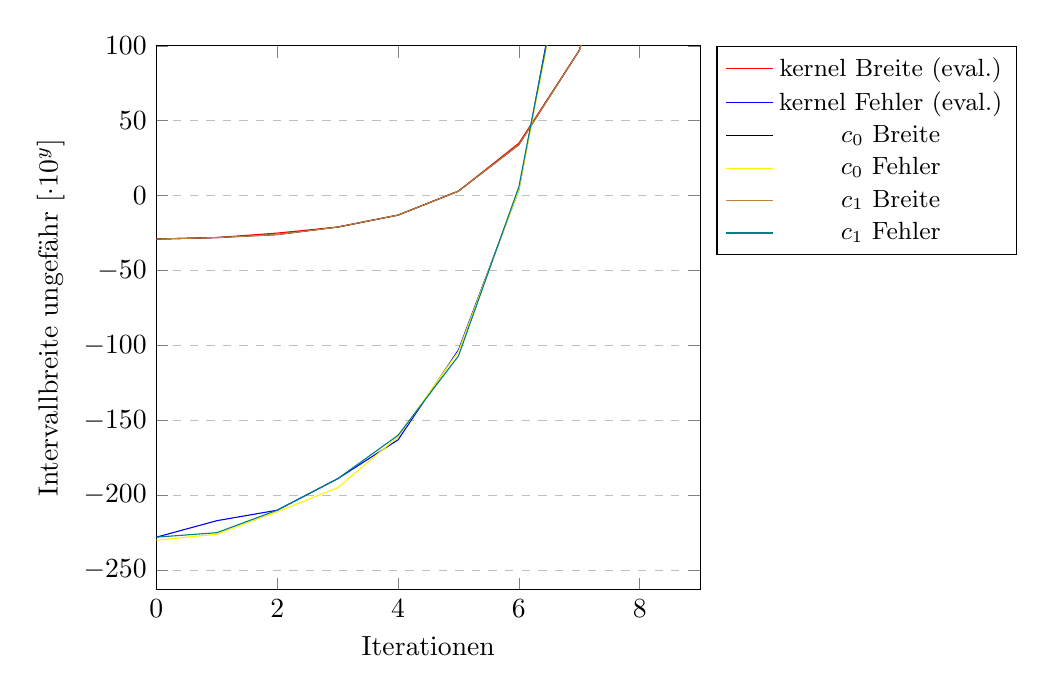
\begin{tikzpicture}
    \begin{axis}[
        width=0.7\textwidth,
        height=0.7\textwidth,
        xlabel={Iterationen},
        ylabel={Intervallbreite ungefähr $[\cdot 10^y ]$},
        legend pos=north west,
        xmin=0,xmax=9,
        ymax=100,
        ymajorgrids=true,
        grid style=dashed,
        legend pos=outer north east,
        cycle list name=color list
    ]
    
    \addplot
        coordinates {
 (0,-29)
 (1,-28)
 (2,-25)
 (3,-21)
 (4,-13)
 (5,03)
 (6,035)
 (7,097)
 (8,0223)
        };
        \addlegendentry{\small{kernel Breite (eval.)}}
    
    \addplot
        coordinates {
  (0,-228)
 (1,-217)
 (2,-210)
 (3,-189)
 (4,-163)
 (5,-103)
 (6,4)
 (7,220)
        };
        \addlegendentry{\small{kernel Fehler (eval.)}}
       
    
    \addplot
        coordinates {
 (0,-29)
 (1,-28)
 (2,-26)
 (3,-21)
 (4,-13)
 (5,03)
 (6,034)
 (7,097)
 (8,0223)
        };
        \addlegendentry{\small{$c_0$ Breite}}
        
    \addplot
        coordinates {
  (0,-230)
 (1,-226)
 (2,-211)
 (3,-195)
 (4,-161)
 (5,-104)
 (6,4)
 (7,212)
 (8,631)
        };
        \addlegendentry{\small{$c_0$ Fehler}}
    
        \addplot
        coordinates {
 (0,-29)
 (1,-28)
 (2,-26)
 (3,-21)
 (4,-13)
 (5,03)
 (6,034)
 (7,097)
 (8,0223)
        };
        \addlegendentry{\small{$c_1$ Breite}}
    
        \addplot
        coordinates {
   (0,-228)
 (1,-225)
 (2,-210)
 (3,-189)
 (4,-160)
 (5,-107)
 (6,6)
 (7,214)
        };
        \addlegendentry{\small{$c_1$ Fehler}}
    
    
    \end{axis}
    \end{tikzpicture}
    \caption{$x_0 = [0 \pm 0] + [0.5 \pm \varepsilon] \cdot \lambda,\  \lambda \in [1 \pm 0]$}
    \label{fig:tm4}
\end{figure}
% 
\begin{figure}[ht]
    \centering
    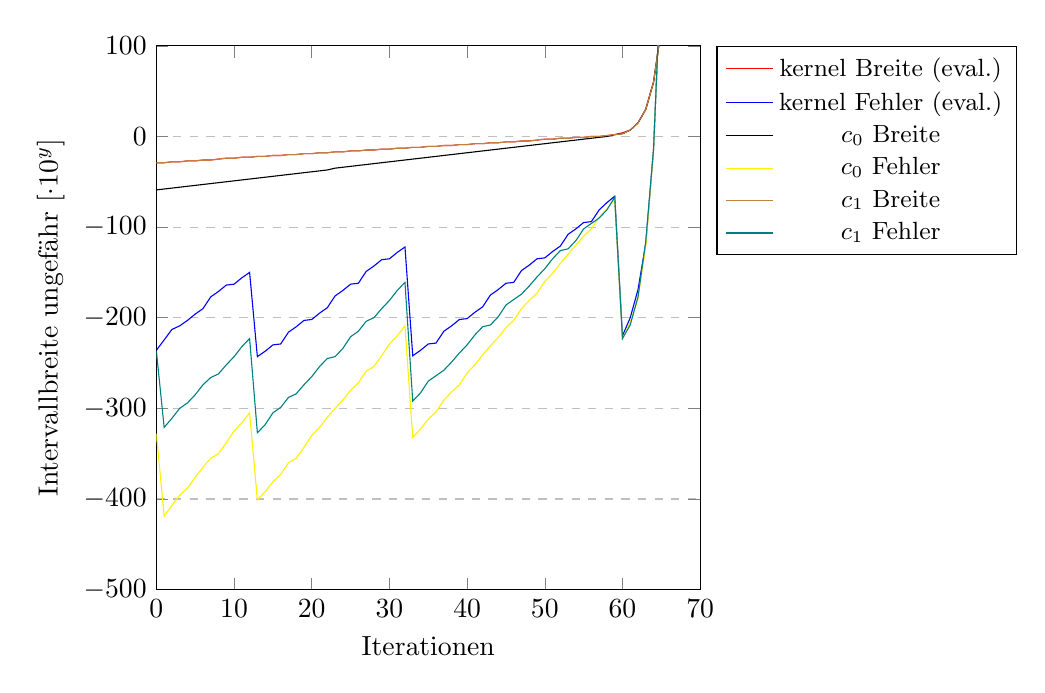
\begin{tikzpicture}
    \begin{axis}[
        width=0.7\textwidth,
        height=0.7\textwidth,
        xlabel={Iterationen},
        ylabel={Intervallbreite ungefähr $[\cdot 10^y ]$},
        legend pos=north west,
        xmin=0,xmax=70,
        ymax=100,ymin=-500,
        ymajorgrids=true,
        grid style=dashed,
        legend pos=outer north east,
        cycle list name=color list
    ]
    
    \addplot
        coordinates {
 (0,-29)
 (1,-29)
 (2,-28)
 (3,-28)
 (4,-27)
 (5,-27)
 (6,-26)
 (7,-26)
 (8,-25)
 (9,-24)
 (10,-24)
 (11,-23)
 (12,-23)
 (13,-22)
 (14,-22)
 (15,-21)
 (16,-21)
 (17,-20)
 (18,-20)
 (19,-19)
 (20,-19)
 (21,-18)
 (22,-18)
 (23,-17)
 (24,-17)
 (25,-16)
 (26,-16)
 (27,-15)
 (28,-15)
 (29,-14)
 (30,-14)
 (31,-13)
 (32,-13)
 (33,-12)
 (34,-12)
 (35,-11)
 (36,-11)
 (37,-10)
 (38,-10)
 (39,-9)
 (40,-9)
 (41,-8)
 (42,-8)
 (43,-7)
 (44,-7)
 (45,-6)
 (46,-6)
 (47,-5)
 (48,-5)
 (49,-4)
 (50,-3)
 (51,-3)
 (52,-2)
 (53,-2)
 (54,-1)
 (55,-1)
 (56,0)
 (57,0)
 (58,01)
 (59,02)
 (60,04)
 (61,07)
 (62,015)
 (63,030)
 (64,060)
 (65,0120)
        };
        \addlegendentry{\small{kernel Breite (eval.)}}
    
    \addplot
        coordinates {
  (0,-236)
 (2,-213)
 (3,-209)
 (4,-203)
 (5,-196)
 (6,-190)
 (7,-177)
 (8,-171)
 (9,-164)
 (10,-163)
 (11,-156)
 (12,-150)
 (13,-243)
 (14,-237)
 (15,-230)
 (16,-229)
 (17,-216)
 (18,-210)
 (19,-203)
 (20,-202)
 (21,-195)
 (22,-189)
 (23,-176)
 (24,-170)
 (25,-163)
 (26,-162)
 (27,-149)
 (28,-143)
 (29,-136)
 (30,-135)
 (31,-128)
 (32,-122)
 (33,-242)
 (34,-236)
 (35,-229)
 (36,-228)
 (37,-215)
 (38,-209)
 (39,-202)
 (40,-201)
 (41,-194)
 (42,-188)
 (43,-175)
 (44,-169)
 (45,-162)
 (46,-161)
 (47,-148)
 (48,-142)
 (49,-135)
 (50,-134)
 (51,-127)
 (52,-121)
 (53,-108)
 (54,-102)
 (55,-95)
 (56,-94)
 (57,-81)
 (58,-73)
 (59,-66)
 (60,-220)
 (61,-200)
 (62,-169)
 (63,-118)
 (64,-14)
 (65,191)
        };
        \addlegendentry{\small{kernel Fehler (eval.)}}
       
    
    \addplot
        coordinates {
 (0,-59)
 (1,-58)
 (2,-57)
 (3,-56)
 (4,-55)
 (5,-54)
 (6,-53)
 (7,-52)
 (8,-51)
 (9,-50)
 (10,-49)
 (11,-48)
 (12,-47)
 (13,-46)
 (14,-45)
 (15,-44)
 (16,-43)
 (17,-42)
 (18,-41)
 (19,-40)
 (20,-39)
 (21,-38)
 (22,-37)
 (23,-35)
 (24,-34)
 (25,-33)
 (26,-32)
 (27,-31)
 (28,-30)
 (29,-29)
 (30,-28)
 (31,-27)
 (32,-26)
 (33,-25)
 (34,-24)
 (35,-23)
 (36,-22)
 (37,-21)
 (38,-20)
 (39,-19)
 (40,-18)
 (41,-17)
 (42,-16)
 (43,-15)
 (44,-14)
 (45,-13)
 (46,-12)
 (47,-11)
 (48,-10)
 (49,-9)
 (50,-8)
 (51,-7)
 (52,-6)
 (53,-5)
 (54,-4)
 (55,-3)
 (56,-2)
 (57,-1)
 (58,0)
 (59,02)
 (60,03)
 (61,07)
 (62,015)
 (63,030)
 (64,060)
 (65,0119)
        };
        \addlegendentry{\small{$c_0$ Breite}}
        
    \addplot
        coordinates {
  (0,-328)
 (1,-419)
 (2,-407)
 (3,-396)
 (4,-388)
 (5,-376)
 (6,-365)
 (7,-355)
 (8,-350)
 (9,-338)
 (10,-325)
 (11,-316)
 (12,-305)
 (13,-401)
 (14,-392)
 (15,-381)
 (16,-373)
 (17,-360)
 (18,-355)
 (19,-343)
 (20,-330)
 (21,-321)
 (22,-310)
 (23,-300)
 (24,-291)
 (25,-280)
 (26,-272)
 (27,-259)
 (28,-254)
 (29,-242)
 (30,-229)
 (31,-220)
 (32,-209)
 (33,-332)
 (34,-323)
 (35,-312)
 (36,-304)
 (37,-291)
 (38,-282)
 (39,-274)
 (40,-261)
 (41,-252)
 (42,-241)
 (43,-231)
 (44,-222)
 (45,-211)
 (46,-203)
 (47,-190)
 (48,-181)
 (49,-173)
 (50,-160)
 (51,-151)
 (52,-140)
 (53,-130)
 (54,-120)
 (55,-110)
 (56,-102)
 (57,-89)
 (58,-80)
 (59,-69)
 (60,-223)
 (61,-205)
 (62,-179)
 (63,-121)
 (64,-15)
 (65,191)
        };
        \addlegendentry{\small{$c_0$ Fehler}}
    
        \addplot
        coordinates {
 (0,-29)
 (1,-29)
 (2,-28)
 (3,-28)
 (4,-27)
 (5,-27)
 (6,-26)
 (7,-26)
 (8,-25)
 (9,-24)
 (10,-24)
 (11,-23)
 (12,-23)
 (13,-22)
 (14,-22)
 (15,-21)
 (16,-21)
 (17,-20)
 (18,-20)
 (19,-19)
 (20,-19)
 (21,-18)
 (22,-18)
 (23,-17)
 (24,-17)
 (25,-16)
 (26,-16)
 (27,-15)
 (28,-15)
 (29,-14)
 (30,-14)
 (31,-13)
 (32,-13)
 (33,-12)
 (34,-12)
 (35,-11)
 (36,-11)
 (37,-10)
 (38,-10)
 (39,-9)
 (40,-9)
 (41,-8)
 (42,-8)
 (43,-7)
 (44,-7)
 (45,-6)
 (46,-6)
 (47,-5)
 (48,-5)
 (49,-4)
 (50,-3)
 (51,-3)
 (52,-2)
 (53,-2)
 (54,-1)
 (55,-1)
 (56,0)
 (57,0)
 (58,01)
 (59,02)
 (60,03)
 (61,07)
 (62,015)
 (63,030)
 (64,060)
 (65,0119)
        };
        \addlegendentry{\small{$c_1$ Breite}}
    
        \addplot
        coordinates {
   (0,-237)
 (1,-321)
 (2,-311)
 (3,-300)
 (4,-294)
 (5,-285)
 (6,-274)
 (7,-266)
 (8,-262)
 (9,-252)
 (10,-243)
 (11,-232)
 (12,-223)
 (13,-327)
 (14,-318)
 (15,-305)
 (16,-299)
 (17,-288)
 (18,-284)
 (19,-274)
 (20,-265)
 (21,-254)
 (22,-245)
 (23,-243)
 (24,-234)
 (25,-221)
 (26,-215)
 (27,-204)
 (28,-200)
 (29,-190)
 (30,-181)
 (31,-170)
 (32,-161)
 (33,-292)
 (34,-283)
 (35,-270)
 (36,-264)
 (37,-258)
 (38,-249)
 (39,-239)
 (40,-230)
 (41,-219)
 (42,-210)
 (43,-208)
 (44,-199)
 (45,-186)
 (46,-180)
 (47,-174)
 (48,-165)
 (49,-155)
 (50,-146)
 (51,-135)
 (52,-126)
 (53,-124)
 (54,-115)
 (55,-102)
 (56,-96)
 (57,-90)
 (58,-81)
 (59,-67)
 (60,-223)
 (61,-208)
 (62,-177)
 (63,-116)
 (64,-14)
 (65,190)

        };
        \addlegendentry{\small{$c_1$ Fehler}}
    
    
    \end{axis}
    \end{tikzpicture}
    \caption{$x_0 = [0.5 \pm 0] + [0 \pm \varepsilon] \cdot \lambda ,\ \lambda \in [1 \pm 0]$}
    \label{fig:tm5}
\end{figure}
% 
\begin{figure}[ht]
    \centering
    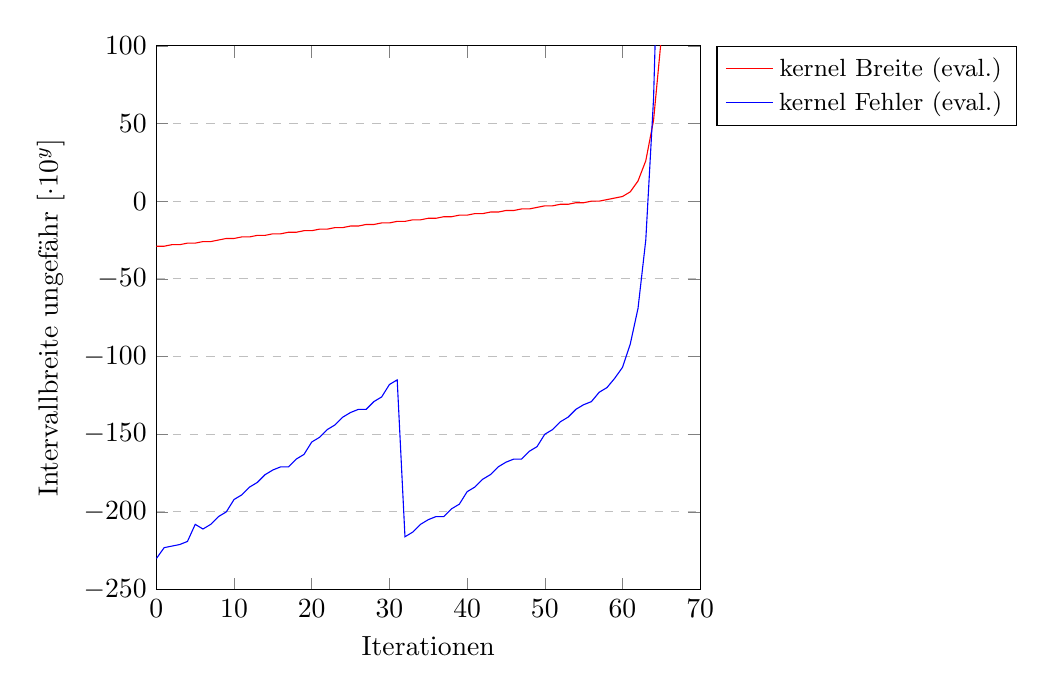
\begin{tikzpicture}
    \begin{axis}[
        width=0.7\textwidth,
        height=0.7\textwidth,
        xlabel={Iterationen},
        ylabel={Intervallbreite ungefähr $[\cdot 10^y ]$},
        legend pos=north west,
        xmin=0,xmax=70,
        ymax=100,ymin=-250,
        ymajorgrids=true,
        grid style=dashed,
        legend pos=outer north east,
        cycle list name=color list
    ]
    
    \addplot
        coordinates {
 (0,-29)
 (1,-29)
 (2,-28)
 (3,-28)
 (4,-27)
 (5,-27)
 (6,-26)
 (7,-26)
 (8,-25)
 (9,-24)
 (10,-24)
 (11,-23)
 (12,-23)
 (13,-22)
 (14,-22)
 (15,-21)
 (16,-21)
 (17,-20)
 (18,-20)
 (19,-19)
 (20,-19)
 (21,-18)
 (22,-18)
 (23,-17)
 (24,-17)
 (25,-16)
 (26,-16)
 (27,-15)
 (28,-15)
 (29,-14)
 (30,-14)
 (31,-13)
 (32,-13)
 (33,-12)
 (34,-12)
 (35,-11)
 (36,-11)
 (37,-10)
 (38,-10)
 (39,-9)
 (40,-9)
 (41,-8)
 (42,-8)
 (43,-7)
 (44,-7)
 (45,-6)
 (46,-6)
 (47,-5)
 (48,-5)
 (49,-4)
 (50,-3)
 (51,-3)
 (52,-2)
 (53,-2)
 (54,-1)
 (55,-1)
 (56,0)
 (57,0)
 (58,01)
 (59,02)
 (60,03)
 (61,06)
 (62,013)
 (63,026)
 (64,052)
 (65,0105)
        };
        \addlegendentry{\small{kernel Breite (eval.)}}
    
    \addplot
        coordinates {
  (0,-230)
 (1,-223)
 (2,-222)
 (3,-221)
 (4,-219)
 (5,-208)
 (6,-211)
 (7,-208)
 (8,-203)
 (9,-200)
 (10,-192)
 (11,-189)
 (12,-184)
 (13,-181)
 (14,-176)
 (15,-173)
 (16,-171)
 (17,-171)
 (18,-166)
 (19,-163)
 (20,-155)
 (21,-152)
 (22,-147)
 (23,-144)
 (24,-139)
 (25,-136)
 (26,-134)
 (27,-134)
 (28,-129)
 (29,-126)
 (30,-118)
 (31,-115)
 (32,-216)
 (33,-213)
 (34,-208)
 (35,-205)
 (36,-203)
 (37,-203)
 (38,-198)
 (39,-195)
 (40,-187)
 (41,-184)
 (42,-179)
 (43,-176)
 (44,-171)
 (45,-168)
 (46,-166)
 (47,-166)
 (48,-161)
 (49,-158)
 (50,-150)
 (51,-147)
 (52,-142)
 (53,-139)
 (54,-134)
 (55,-131)
 (56,-129)
 (57,-123)
 (58,-120)
 (59,-114)
 (60,-107)
 (61,-92)
 (62,-69)
 (63,-25)
 (64,66)
 (65,241)
        };
        \addlegendentry{\small{kernel Fehler (eval.)}}
      
    
    \end{axis}
    \end{tikzpicture}
    \caption{$x_0 = [0.5 \pm \varepsilon]$}
    \label{fig:tm6}
\end{figure}
%
\begin{figure}[ht]
    \centering
    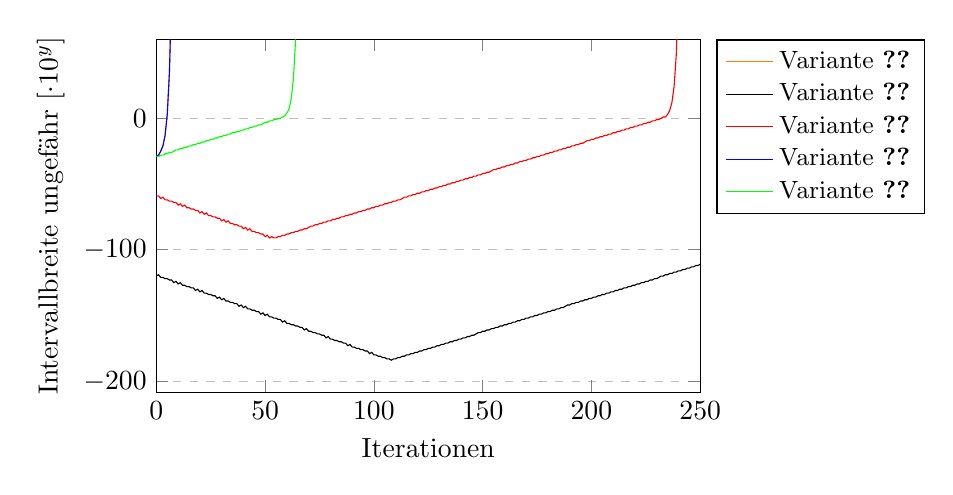
\begin{tikzpicture}
    \begin{axis}[
        width=0.7\textwidth,
        height=0.5\textwidth,
        xlabel={Iterationen},
        ylabel={Intervallbreite ungefähr $[\cdot 10^y ]$},
        legend pos=north west,
        xmin=0,xmax=250,
        ymax=60,
        ymajorgrids=true,
        grid style=dashed,
        legend pos=outer north east
    ]
    
    \addplot[
        color=orange,
        ]
        coordinates {
    (0,-29)
(1,-28)
(2,-25)
(3,-21)
(4,-13)
(5,03)
(6,35)
(7,97)
(8,223)
        };
        \addlegendentry{\small{Variante \ref{tm1}}}
    
    \addplot[
        color=black,
        ]
        coordinates {
    (0,-120) (1,-119) (2,-121) (3,-121) (4,-122) (5,-122) (6,-123) (7,-123) (8,-125) (9,-124) (10,-126) (11,-125) (12,-127) (13,-127) (14,-128) (15,-128) (16,-129) (17,-129) (18,-131) (19,-130) (20,-132) (21,-131) (22,-133) (23,-133) (24,-134) (25,-134) (26,-135) (27,-135) (28,-137) (29,-136) (30,-138) (31,-137) (32,-139) (33,-139) (34,-140) (35,-140) (36,-141) (37,-141) (38,-143) (39,-142) (40,-144) (41,-143) (42,-145) (43,-145) (44,-146) (45,-146) (46,-147) (47,-147) (48,-149) (49,-148) (50,-150) (51,-149) (52,-151) (53,-151) (54,-152) (55,-152) (56,-153) (57,-153) (58,-155) (59,-154) (60,-156) (61,-156) (62,-157) (63,-157) (64,-158) (65,-158) (66,-159) (67,-159) (68,-161) (69,-160) (70,-162) (71,-162) (72,-163) (73,-163) (74,-164) (75,-164) (76,-165) (77,-165) (78,-167) (79,-166) (80,-168) (81,-168) (82,-169) (83,-169) (84,-170) (85,-170) (86,-171) (87,-171) (88,-173) (89,-172) (90,-174) (91,-174) (92,-175) (93,-175) (94,-176) (95,-176) (96,-177) (97,-177) (98,-179) (99,-178) (100,-180) (101,-180) (102,-181) (103,-181) (104,-182) (105,-182) (106,-183) (107,-183) (108,-184) (109,-183) (110,-183) (111,-182) (112,-182) (113,-181) (114,-181) (115,-180) (116,-180) (117,-179) (118,-179) (119,-178) (120,-178) (121,-177) (122,-177) (123,-176) (124,-176) (125,-175) (126,-175) (127,-174) (128,-174) (129,-173) (130,-173) (131,-172) (132,-172) (133,-171) (134,-171) (135,-170) (136,-170) (137,-169) (138,-169) (139,-168) (140,-168) (141,-167) (142,-167) (143,-166) (144,-166) (145,-165) (146,-165) (147,-164) (148,-163) (149,-163) (150,-162) (151,-162) (152,-161) (153,-161) (154,-160) (155,-160) (156,-159) (157,-159) (158,-158) (159,-158) (160,-157) (161,-157) (162,-156) (163,-156) (164,-155) (165,-155) (166,-154) (167,-154) (168,-153) (169,-153) (170,-152) (171,-152) (172,-151) (173,-151) (174,-150) (175,-150) (176,-149) (177,-149) (178,-148) (179,-148) (180,-147) (181,-147) (182,-146) (183,-146) (184,-145) (185,-145) (186,-144) (187,-144) (188,-143) (189,-142) (190,-142) (191,-141) (192,-141) (193,-140) (194,-140) (195,-139) (196,-139) (197,-138) (198,-138) (199,-137) (200,-137) (201,-136) (202,-136) (203,-135) (204,-135) (205,-134) (206,-134) (207,-133) (208,-133) (209,-132) (210,-132) (211,-131) (212,-131) (213,-130) (214,-130) (215,-129) (216,-129) (217,-128) (218,-128) (219,-127) (220,-127) (221,-126) (222,-126) (223,-125) (224,-125) (225,-124) (226,-124) (227,-123) (228,-123) (229,-122) (230,-122) (231,-121) (232,-120) (233,-120) (234,-119) (235,-119) (236,-118) (237,-118) (238,-117) (239,-117) (240,-116) (241,-116) (242,-115) (243,-115) (244,-114) (245,-114) (246,-113) (247,-113) (248,-112) (249,-112) (250,-111)
        };
        \addlegendentry{\small{Variante \ref{tm2}}}
        
    \addplot[
        color=red,
        ]
        coordinates {
    (0,-59) (1,-59) (2,-61) (3,-60) (4,-62) (5,-62) (6,-63) (7,-63) (8,-64) (9,-64) (10,-66) (11,-65) (12,-67) (13,-66) (14,-68) (15,-68) (16,-69) (17,-69) (18,-70) (19,-70) (20,-72) (21,-71) (22,-73) (23,-72) (24,-74) (25,-74) (26,-75) (27,-75) (28,-76) (29,-76) (30,-78) (31,-77) (32,-79) (33,-78) (34,-80) (35,-80) (36,-81) (37,-81) (38,-82) (39,-82) (40,-84) (41,-83) (42,-85) (43,-84) (44,-86) (45,-86) (46,-87) (47,-87) (48,-88) (49,-88) (50,-90) (51,-89) (52,-91) (53,-90) (54,-91) (55,-91) (56,-90) (57,-90) (58,-89) (59,-89) (60,-88) (61,-88) (62,-87) (63,-87) (64,-86) (65,-86) (66,-85) (67,-85) (68,-84) (69,-84) (70,-83) (71,-82) (72,-82) (73,-81) (74,-81) (75,-80) (76,-80) (77,-79) (78,-79) (79,-78) (80,-78) (81,-77) (82,-77) (83,-76) (84,-76) (85,-75) (86,-75) (87,-74) (88,-74) (89,-73) (90,-73) (91,-72) (92,-72) (93,-71) (94,-71) (95,-70) (96,-70) (97,-69) (98,-69) (99,-68) (100,-68) (101,-67) (102,-67) (103,-66) (104,-66) (105,-65) (106,-65) (107,-64) (108,-64) (109,-63) (110,-63) (111,-62) (112,-62) (113,-61) (114,-60) (115,-60) (116,-59) (117,-59) (118,-58) (119,-58) (120,-57) (121,-57) (122,-56) (123,-56) (124,-55) (125,-55) (126,-54) (127,-54) (128,-53) (129,-53) (130,-52) (131,-52) (132,-51) (133,-51) (134,-50) (135,-50) (136,-49) (137,-49) (138,-48) (139,-48) (140,-47) (141,-47) (142,-46) (143,-46) (144,-45) (145,-45) (146,-44) (147,-44) (148,-43) (149,-43) (150,-42) (151,-42) (152,-41) (153,-41) (154,-40) (155,-39) (156,-39) (157,-38) (158,-38) (159,-37) (160,-37) (161,-36) (162,-36) (163,-35) (164,-35) (165,-34) (166,-34) (167,-33) (168,-33) (169,-32) (170,-32) (171,-31) (172,-31) (173,-30) (174,-30) (175,-29) (176,-29) (177,-28) (178,-28) (179,-27) (180,-27) (181,-26) (182,-26) (183,-25) (184,-25) (185,-24) (186,-24) (187,-23) (188,-23) (189,-22) (190,-22) (191,-21) (192,-21) (193,-20) (194,-20) (195,-19) (196,-19) (197,-18) (198,-17) (199,-17) (200,-16) (201,-16) (202,-15) (203,-15) (204,-14) (205,-14) (206,-13) (207,-13) (208,-12) (209,-12) (210,-11) (211,-11) (212,-10) (213,-10) (214,-9) (215,-9) (216,-8) (217,-8) (218,-7) (219,-7) (220,-6) (221,-6) (222,-5) (223,-5) (224,-4) (225,-4) (226,-3) (227,-3) (228,-2) (229,-2) (230,-1) (231,-1) (232,00) (233,01) (234,01) (235,03) (236,06) (237,12) (238,24) (239,48) (240,96)
        };
        \addlegendentry{\small{Variante \ref{tm3}}}
    
    
    \addplot[
        color=blue,
        ]
        coordinates {
    (0,-29) (1,-28) (2,-25) (3,-21) (4,-13) (5,03) (6,35) (7,97)
        };
        \addlegendentry{\small{Variante \ref{tm4}}}
    
    \addplot[
        color=green,
        ]
        coordinates {
    (0,-29) (1,-29) (2,-28) (3,-28) (4,-27) (5,-27) (6,-26) (7,-26) (8,-25) (9,-24) (10,-24) (11,-23) (12,-23) (13,-22) (14,-22) (15,-21) (16,-21) (17,-20) (18,-20) (19,-19) (20,-19) (21,-18) (22,-18) (23,-17) (24,-17) (25,-16) (26,-16) (27,-15) (28,-15) (29,-14) (30,-14) (31,-13) (32,-13) (33,-12) (34,-12) (35,-11) (36,-11) (37,-10) (38,-10) (39,-9) (40,-9) (41,-8) (42,-8) (43,-7) (44,-7) (45,-6) (46,-6) (47,-5) (48,-5) (49,-4) (50,-3) (51,-3) (52,-2) (53,-2) (54,-1) (55,-1) (56,00) (57,00) (58,01) (59,02) (60,04) (61,07) (62,15) (63,30) (64,60)
        };
        \addlegendentry{\small{Variante \ref{tm5}}}
                                      
    
    
    
    
    \end{axis}
    \end{tikzpicture}
    \caption{Größenordnung der Breite des Kernintervalls bei der Berechnung von $x_{250}$ mit Sweeping square\_only mit unterschiedlichen Definitionen des Taylormodells für $x_0$}
    \label{fig:strategy2}
\end{figure}


%% ==============================
\label{ch:Evaluierung:sec:zusammenfassung}


%%% Local Variables: 
%%% mode: latex
%%% TeX-master: "thesis"
%%% End: 

